\section{Towards Real-Time System}
\label{sec:volumetric:rts}
\begin{figure}[!htb]
\centering
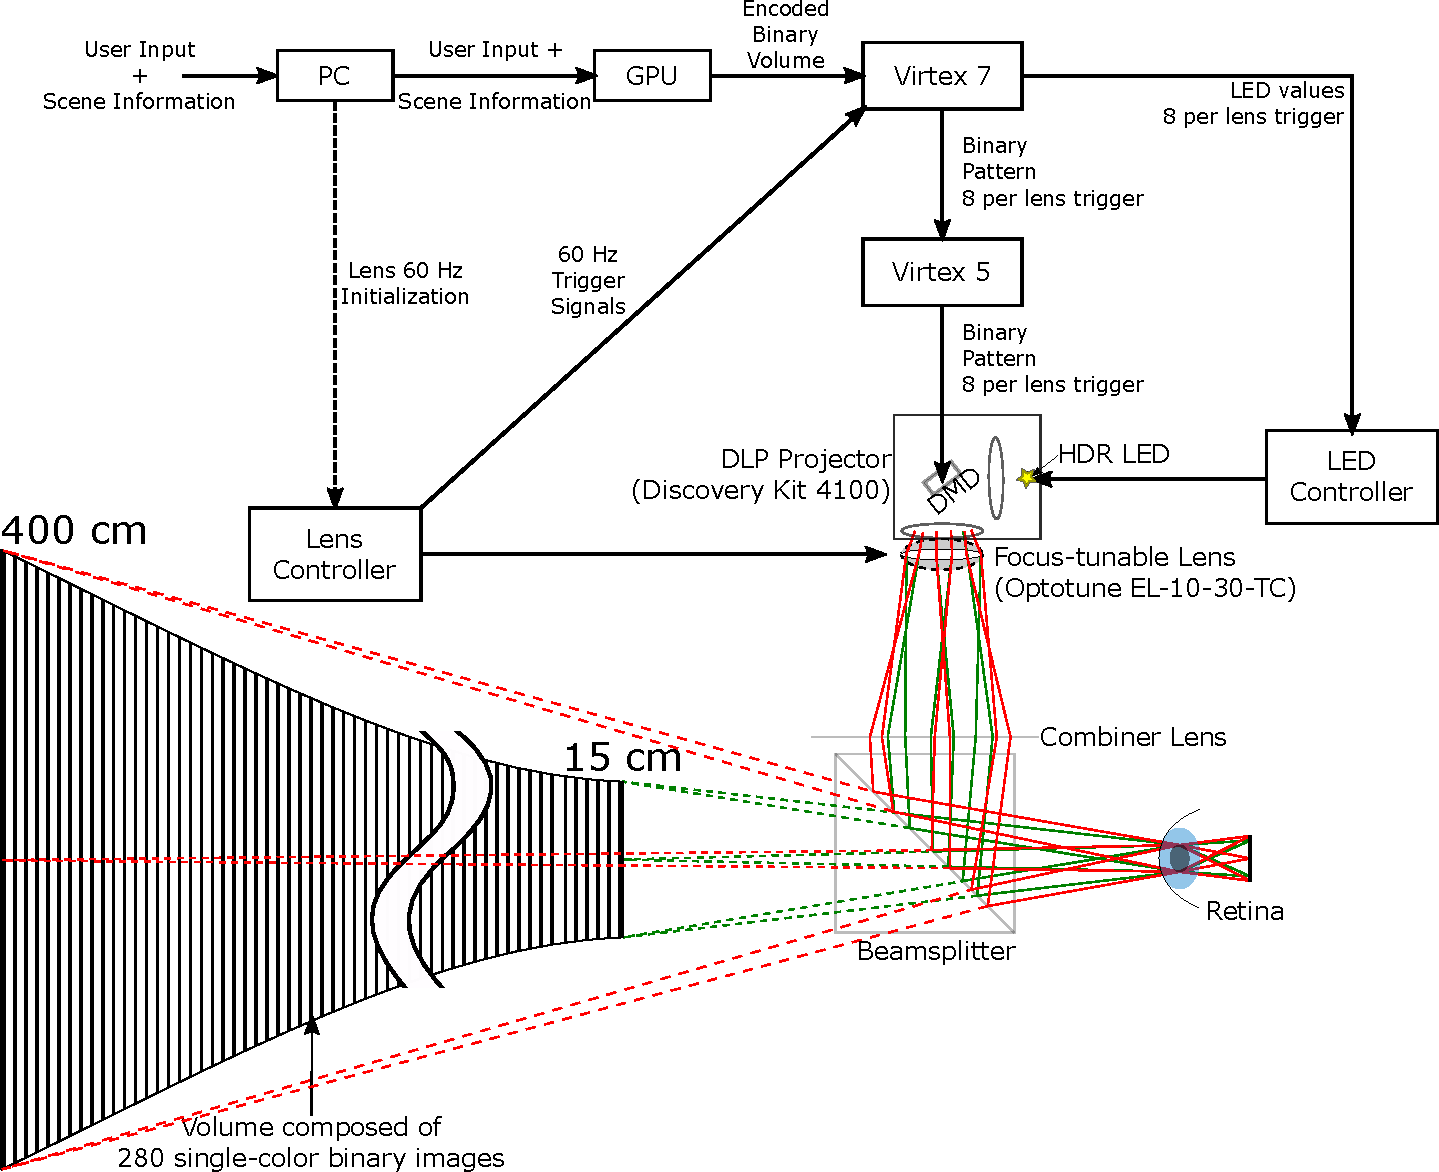
\includegraphics[width=0.99\columnwidth]{images/volumetric/real_time_system/real_time_system_overview}
\caption[Volumetric NED: Overview of real-time display system]{Figure shows the overview of the real-time volumetric display system.}
\label{fig:volumetric:rts:overview}
\end{figure}



A real-time system with only 8 depth planes was developed as part of this dissertation to demonstrate the future feasibility of a completely developed real-time system.
Fig.~\ref{fig:volumetric:rts:overview} shows an overview of the real-time volumetric display system.
In Fig.~\ref{fig:volumetric:rts:overview}, solid lines indicate real-time tasks and dashed lines indicate off-line tasks.
The only off-line task is to initialize the lens driver to oscillate the focal length of the lens at 60 Hz. 
The computational compoenents of this real-time system and their tasks is summarized below:

\begin{enumerate}
    \item PC:
    \begin{itemize}
        \item Initializes the lens driver to oscillate at 60 Hz. 
        \item Passes scene infomration (3D models, lighting information, camera position) to the GPU.
        \item Interprets user mouse movements to modify camera position.
    \end{itemize}
    \item GPU (in the order mentioned):
    \begin{itemize}
        \item Render 3D scene into an RGB image and depth map.
        \item Decomposes RGB image and depth map into 8 binary images and 8 LED colors.
        \item Encodes these 8 binary images into a gray-scale image and copies this gray-scale image into the three color channels of the image being sent over DVI to the Virtex-7 FPGA.
    \end{itemize}
    \item Virtex-7 FPGA:
    \begin{itemize}
        \item Receives the DVI image and stores into an on-board RAM.
        \item Copies two color channels of the image on the RAM onto the cache memory.
        \item Waits for trigger signal from the focus-tunable lens driver which indicates the start of a lens cycle.
        \item Sends 8 RGB LED values to the custom LED controller. These 8 values are uniformely spaced temporally over the duration of one lens cycle assuming that the lens is oscillating at 60 Hz.
        \item Sends 8 binary patterns to the Virtex 5 DMD controller board. These 8 values are uniformely spaced temporally over the duration of one lens cycle assuming that the lens is oscillating at 60 Hz.
    \end{itemize}
\end{enumerate}

\subsection{GPU computation}
\begin{figure}[h!]
\centering
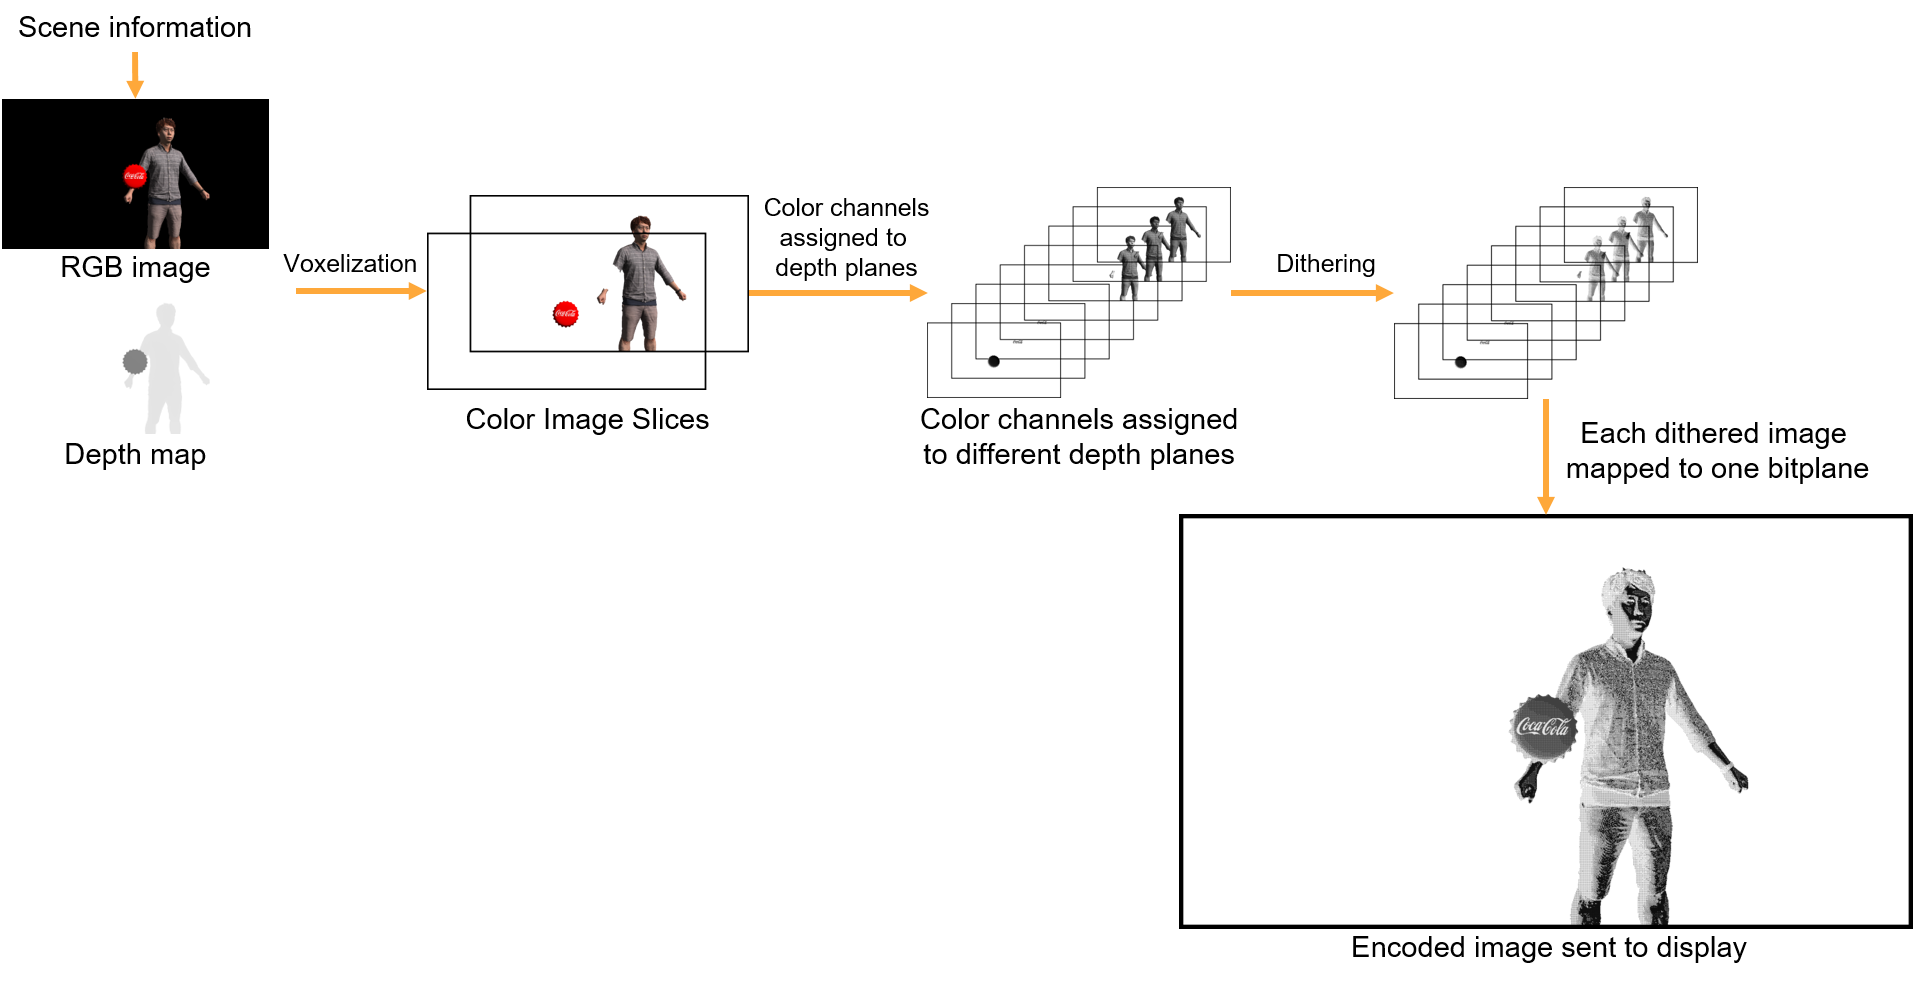
\includegraphics[width=0.99\columnwidth]{images/volumetric/real_time_system/real_time_system_gpu_pipeline}
\caption[GPU pipeline for real-time volumetric display]{Figure shows the GPU computation pipeline for the real-time volumetric display.}
\label{fig:volumetric:rts:gpu_pipeline}
\end{figure}


For this system, we use the fixed-pipeline decomposition scheme and allocate the RGB LED colors of the 8 depth planes to be $L_1 = \{\alpha, 0, 0\}, L_2 = \{0, \alpha, 0\}, L_3 = \{0, 0, \alpha\}, L_4 = \{0, 0, 0,\}, L_5 = \{0, 0, 0\}, L_6 = \{\alpha, 0,0\}, L_7 = \{0, \alpha,0\}, L_8 = \{0, 0, \alpha\}$, where $\alpha$ is some light intensity.

Fig.~\ref{fig:volumetric:rts:gpu_pipeline} shows the GPU computation pipeline for the real-time volumetric display system. Assuming that we are dealing with only opaque objects, we start with rendering the RGB image and depth map of the scene.

From the RGB image and depth map, we calculate the color volume by quantizing the depth values into either the near depth plane or the far depth plane.
For each color depth plane, we split the RGB image into its three color components and assign each color component to one depth plane. 
If $C_1$ is the near depth plane, then the red channel of $C_1$ is assigned to the nearest depth plane, the green channel of $C_1$ is assigned to the second depth plane, and the blue channel of $C_1$ is assigned to the third depth plane and so on.
At this stage, note that each depth plane is still assgined an 8-bit color image.
We rather need binary images at each depth plane so that it is compatible with our system. 
If we had a system with a large number of depth planes like our static volumetric display, each of these color depth planes could be decomposed into 8 binary depth planes.
Since we don't have that, we perform spatial dithering to convert each 8-bit color image into a binary image. 
After this step, we have 8 1-bit images for each depth plane which can be encoded into a single color channel, either red, green, or blue.
Due to some limitations in our FPGA implementation (described in Sec.~\ref{sec:volumetric:rts:limitations}), we copy this encoded image into all the three color channels to make the subsequent parts of the display pipeline agnostic to the color channel it chooses to display.

\subsection{Results}
A video was recorded as demonstration of this real-time volumetric display system. This video was submitted as part of this dissertation and is also available publically at this URL: \url{https://www.youtube.com/watch?v=pUtvBEPkzfA}. 
The video shows two real objects and two virtual objects. 
The real objects are a postage stamp at 30 cm and a real person at 300 cm.
The virtual objects are a Coca-Cola bottle cap model and a 3D body scan of a person.
To demonstrate the real-time nature of the system, the real person was asked to juggle some balls.
To demonstrate the interactiveness of the system, the AR objects are rotated during the recording.
To demonsrate the volumetric nature of the system, the camera's focus is changed graduatually between far and near focus settings bringing different parts of the scene into focus.

As we can see, the resolution and colors of the AR body model are severly compromised due to our system's limitations which reduces a 3-channel 8-bits-per-channel color volume to a 3-channel 1-bit-per-channel binary volume.
The visual quality of the AR scene can be significantly improved by increasing the number of binary planes of the system and by using more sophisticated decomposition schemes as explored in Section~\ref{sec:volumetric:acd}.

\subsection{Current limitations}
\label{sec:volumetric:rts:limitations}
The Virtex-7 FPGA program used here is a slightly modified version of Lincoln et al.'s scene-adaptive low-latency AR display~\cite{Lincoln2017scene}.
The modifications include (1) listening for the trigger from the lens driver, (2) modified timings to output only 8 binary images in $\frac{1}{60}$-th of a second.
As mentioned above, one of the Virtex-7 FPGA's activities is to transfer two color channels of the received image from the RAM to the cache memory.
In doing so, it may choose to transfer either Red and Green, or Green and Blue, or Blue and Red.
The order did not matter in \cite{Lincoln2017scene}'s work but it matters for our system because the images shown within one lens cycle's duration need to be in a fixed and pre-determined order. 
However, we didn't implement the necessary modificatins to ensure a deterministic order of copying the color channels and instead chose to make the system color channel agnostic by copying the same gray-scale image into the three color channels of the image. 
If this modification were done, the number of binary planes would be 24 instead of 8.


